% !TeX root = ../../Book5.tex
% * 状态：初稿已完成；正文、证明、算例与配套习题解答已写齐，尚未正式审核。
% 纲要标题：## 附录 F　有限 Lie 型群初步

\chapter{有限 Lie 型群初步}
\label{b5:app:F}
\BookChapterNumber{b5:app:F}

\begin{chapterabstract}
	有限域上的经典群既是有限矩阵群，也是代数群在 Frobenius 映射下的不动点。本附录从这些具体模型出发，用两个旗的共同适配基证明一般线性群的 Bruhat 分解与 BN 对公理，再把旗组织成楼的公寓和室。对群阶、邻旗与双陪集的计数分别给出显式 Sylow 子群和 Hecke 代数的乘法；低秩算例说明这些结构如何进入表示计算。
\end{chapterabstract}

\begin{learninggoals}
	\begin{itemize}
		\item 区分保持交替型、二次型和 Hermitian 型的条件，并核验分裂与酉群的 Frobenius 不动点模型。
		\item 计算矩阵根子群的共轭与交换子，说明它们与有限域加法群的关系。
		\item 从两个旗的交维数恢复相对位置，证明一般线性群的 Bruhat 分解，并计算部分旗的双陪集。
		\item 在旗复形中辨认公寓、室和余维一面，验证向量空间的旗楼公理及低秩邻接关系。
		\item 通过数基与数旗求 \(\operatorname{GL}_n\)、\(\operatorname{SL}_n\) 与 \(\operatorname{Sp}_{2m}\) 的阶，构造定义特征的 Sylow 子群，并求 Hecke 乘法系数。
	\end{itemize}
\end{learninggoals}

\(\operatorname{GL}_3(\mathbb F_2)\) 有 \(168\) 个元素，却只作用在 \(21\) 个完全旗上。固定一个旗后，其他旗按相对位置分成六类；对每一类求和，得到六个与群作用相容的线性算子。为什么位置类型的数目恰好是 \(3!\)，这些算子的乘法又为什么只含有限域大小所决定的系数？回答这两个问题，需要把矩阵的行列变换与子空间的包含关系放在一起研究。

\ProseParagraphBreak
\secref{b5:sec:F01}先建立有限域上的群模型，特别区分群的定义域与以后表示空间的系数域。\secref{b5:sec:F02}通过同时适配两个旗的基，把相对位置化为置换；这也给出 BN 对在一般线性群中的完整验证。\secref{b5:sec:F03}将同一组旗看成单纯复形，公寓则来自一组坐标直线。最后，\secref{b5:sec:F04}用邻旗计数解释 Hecke 代数参数，并计算秩一表示的常值与增广部分。这里直接证明的是经典群的具体构造和一般线性群的旗模型；不以这些算例代替全部有限 Lie 型群的分类。

\ProseParagraphBreak
预备知识包括第一卷的有限域与 Sylow 定理、第二卷的交替型和二次型，以及本卷的置换表示。\chapref{b5:ch:16}的根系与\chapref{b5:ch:21}的代数群提供背景，但矩阵根子群的公式均在本附录重新核验。与抽象 Hecke 代数的同构使用\appref{b5:app:A}中的标准基定理；Bruhat 分解及旗楼的证明只用线性代数和置换长度。

\ProseParagraphBreak
经典群与 BN 对可参阅 Taylor 的专著\cite{Taylor1992ClassicalGroups}。本附录的定位采用作者于2021年修订的公开稿：第四章的群阶公式见第19页，第五章的 BN 对与 Bruhat 分解见第27--36页，第八章的辛基及群阶见第69--70页，第九章的复形与楼见第97--101页。以下证明保留本书的列向量、左作用及 Hermitian 型约定，引用的页码不与1992年刊本混用。

% !TeX root = ../../Book5.tex
% 纲要标题：### F.1 经典群与 Frobenius 映射
% 纲要位置：工作记录/计划纲要.md（2026-10-20 新增骨架）。
% 写作状态：2026-10-20 新增骨架；正文、证明、算例与习题均待撰写。
% 写作范围：以经典群、旗与小秩计算为范围，不展开一般群概形构造、楼的完整理论及 Deligne–Lusztig 理论。
% #### F.1.1 有限域上的经典群
% #### F.1.2 Frobenius 映射与不动点
% #### F.1.3 根子群与分裂群的例子

\section{经典群与 Frobenius 映射}
\label{b5:sec:F01}

待撰写。

\subsection{有限域上的经典群}
\label{b5:subsec:F01:01}

待撰写。

\subsection{Frobenius 映射与不动点}
\label{b5:subsec:F01:02}

待撰写。

\subsection{根子群与分裂群的例子}
\label{b5:subsec:F01:03}

待撰写。

% 新增结构与纲要同步；以下条目均为待撰写计划。
% * 状态：待撰写；当前仅有结构占位。

% !TeX root = ../../Book5.tex
% * 状态：初稿已完成；正文、证明、算例与配套习题解答已写齐，尚未正式审核。
% 纲要标题：### F.2 BN 对与 Bruhat 分解
% 写作状态：初稿已完成；新增内容尚未正式审核。
% #### F.2.1 BN 对的定义
% #### F.2.2 一般线性群的 Bruhat 分解
% #### F.2.3 抛物子群与双陪集

\section{BN 对与 Bruhat 分解}
\label{b5:sec:F02}

对矩阵同时作行变换与列变换，通常能把它化成很简单的形式。如果只允许上三角矩阵给出的变换，就不能任意交换坐标；剩下的置换恰好记录两个完全旗的相对位置。Bruhat 分解把这个观察写成双陪集分解，BN 对则保留其中能够推广到其他群的乘法规律。下面用一般线性群完整建立这一模型，再把完全旗换成只保留若干维数的部分旗。

\subsection{BN 对的定义}
\label{b5:subsec:F02:01}

一个子群的双陪集通常没有简单的乘法：两个双陪集相乘，可能得到许多个双陪集的并。BN 对要求存在一组特别的双陪集，使它们与任意双陪集相乘时，最多产生两个候选位置。这里的有限选择对应于旗中只改动一个子空间。

\begin{definition}\label{b5:def:F-BN-pair}
	设 \(G\) 为群，\(B,N\le G\)，令 \(T=B\cap N\)。假设 \(T\triangleleft N\)，商群 \(W=N/T\) 有一个由阶为二的元素组成的生成集 \(S\)。对 \(w\in W\) 任取提升 \(n_w\in N\)。若
	\begin{enumerate}
		\item \(G=\langle B,N\rangle\)；
		\item 对任意 \(w\in W\) 与 \(s\in S\)，有
		\[
			n_sBn_w\subseteq Bn_{sw}B\cup Bn_wB;
		\]
		\item 对任意 \(s\in S\)，有 \(n_sBn_s^{-1}\not\subseteq B\)，
	\end{enumerate}
	则称 \((B,N)\) 连同上述 \(S\) 为 \(G\) 的一个 \term[BN-dui]{BN 对}[BN-pair]。商群 \(W\) 称为该 BN 对的 Weyl 群，\(S\) 中的元素称为简单反射。
\end{definition}
\symidx{\((B,N)\)：BN 对}
\symidx{\(W=N/(B\cap N)\)：BN 对的 Weyl 群}

因为 \(T\subseteq B\) 且 \(T\triangleleft N\)，双陪集 \(Bn_wB\) 不依赖提升的选择。第二项中的 \(n_sBn_w\) 及第三项中的共轭子群也不因更换提升而改变。最后一项排除简单反射只在 \(B\) 内部重新排列的退化情况；第二项则使逐次乘以简单反射的过程可以追踪。这组公理可与\cite[Chapter 5, p. 27]{Taylor1992ClassicalGroups}对照；下面从旗的交维数建立矩阵群的分解。

\ProseParagraphBreak
以下固定 \(G=\mathrm{GL}_n(\mathbb F_q)\)，\(n\ge2\)，并取
\[
	\begin{aligned}
		B&=\{\text{可逆上三角矩阵}\},\\
		N&=\{\text{每行、每列恰有一个非零元的矩阵}\},\\
		T&=\{\operatorname{diag}(t_1,\ldots,t_n):t_i\in\mathbb F_q^\times\}.
	\end{aligned}
\]
\(N\) 中的矩阵称为\term[danxiang-juzhen]{单项矩阵}[monomial matrix]。它置换坐标直线，因而给出满同态 \(N\to S_n\)，核为 \(T\)。上三角单项矩阵必为对角矩阵，故 \(T=B\cap N\)，并且 \(W=N/T\simeq S_n\)。取 \(S=\{s_i=(i,i+1):1\le i<n\}\)，以及满足
\[
	n_we_j=e_{w(j)}
\]
的置换矩阵 \(n_w\)。这里 \(n_un_w=n_{uw}\)，置换乘法为先作右边的置换。由\subsecref{b5:subsec:A01:01}，\((S_n,S)\) 是 \(A_{n-1}\) 型 Coxeter 系统。BN 对中尚需核验的生成条件与乘法条件，将由旗的相对位置直接给出。

\subsection{一般线性群的 Bruhat 分解}
\label{b5:subsec:F02:02}

设 \(V\) 为 \(n\) 维向量空间。一个\term[wanquan-qi]{完全旗}[complete flag]是子空间链
\[
	0=F_0\subset F_1\subset\cdots\subset F_n=V,
	\qquad \dim F_i=i.
\]
只保留某些中间维数，得到\term[bufen-qi]{部分旗}[partial flag]。在 \(V=\mathbb F_q^n\) 中，记标准完全旗为 \(E_i=\operatorname{span}(e_1,\ldots,e_i)\)。一个可逆矩阵保持全部 \(E_i\)，当且仅当第 \(j\) 列属于 \(E_j\)，也就是矩阵上三角。因此 \(B\) 恰为标准旗的稳定子群。每个完全旗都有适配基，故
\[
	G/B\longrightarrow\{\,V\;\text{中的完全旗}\,\},\qquad gB\longmapsto gE
\]
是 \(G\) 等变双射。这里使用左陪集，左乘 \(G\) 对应对旗的自然作用。

两个旗可以共用一组基，但一般必须用不同的顺序排列这组基。下面的构造同时解释这个事实和所需置换的唯一性。

\begin{lemma}\label{b5:lem:F-common-flag-basis}
	设 \(V\) 为域 \(k\) 上的有限维向量空间，\(0=F_0\subset\cdots\subset F_a=V\) 与 \(0=F'_0\subset\cdots\subset F'_b=V\) 为两个旗。存在子空间 \(C_{ij}\) 使
	\[
		F_i\cap F'_j=\bigoplus_{u\le i,\,v\le j}C_{uv}.
	\]
	尤其有一组基同时适配两个旗。若两旗均为完全旗且 \(\dim V=n\)，则存在唯一 \(w\in S_n\) 满足
	\begin{equation}\label{b5:eq:F-relative-position-ranks}
		r_{ij}\coloneqq\dim(F_i\cap F'_j)=\#\{a\le j:w(a)\le i\}.
	\end{equation}
	此时可取基 \(v_1,\ldots,v_n\) 使 \(F_i=\operatorname{span}(v_1,\ldots,v_i)\)，且 \(F'_j=\operatorname{span}(v_{w(1)},\ldots,v_{w(j)})\)。
\end{lemma}
\begin{proof}
	令 \(V_{ij}=F_i\cap F'_j\)。按 \(i+j\) 递增，选取补空间
	\[
		V_{ij}=(V_{i-1,j}+V_{i,j-1})\oplus C_{ij}.
	\]
	边界 \(V_{0j}=V_{i0}=0\)。由于
	\[
		V_{i-1,j}\cap V_{i,j-1}=V_{i-1,j-1},
	\]
	若两个前驱空间已经由相应的 \(C_{uv}\) 直和表示，它们的和只把共有的项保留一次，再加入 \(C_{ij}\) 就得到所需直和。由归纳，公式对所有 \(i,j\) 成立。每个 \(C_{ij}\) 选一组基，其并即同时适配两旗。

	在完全旗情形，令
	\[
		c_{ij}=\dim C_{ij}
		=r_{ij}-r_{i-1,j}-r_{i,j-1}+r_{i-1,j-1}.
	\]
	这些数非负，而每行的和为 \(\dim F_i-\dim F_{i-1}=1\)，每列的和也为一。因此 \((c_{ij})\) 是一个置换矩阵：第 \(j\) 列唯一的 \(1\) 所在行记为 \(w(j)\)。交维数由它的左上矩形求和给出，故满足\eqref{b5:eq:F-relative-position-ranks}。反过来，上述差分式从交维数唯一恢复 \(c_{ij}\)，从而恢复 \(w\)。在一维空间 \(C_{w(j),j}\) 中选取非零向量并记为 \(v_{w(j)}\)，便得到所述基。
\end{proof}

上述唯一置换记为 \(\operatorname{pos}(F,F')\)，称为两旗的\term[xiangdui-weizhi]{相对位置}[relative position]。同时作用一个线性同构不改变交维数，因而不改变相对位置。由定义也有 \(\operatorname{pos}(F',F)=\operatorname{pos}(F,F')^{-1}\)。
\symidx{\(\operatorname{pos}(F,F')\)：两个完全旗的相对位置}

\begin{theorem}[一般线性群的 Bruhat 分解]\label{b5:thm:F-GL-Bruhat}
	设 \(n\ge1\)，\(G=\mathrm{GL}_n(\mathbb F_q)\)，\(B\) 为可逆上三角子群，\(n_w e_j=e_{w(j)}\)。则
	\[
		G=\bigsqcup_{w\in S_n}Bn_wB.
	\]
	其中 \(g\in Bn_wB\) 当且仅当 \(\operatorname{pos}(E,gE)=w\)。若 \(\ell(w)\) 为 \(w\) 关于相邻换位的长度，则
	\begin{equation}\label{b5:eq:F-Bruhat-cell-size}
		|Bn_wB/B|=q^{\ell(w)},\qquad
		|Bn_wB|=|B|q^{\ell(w)}.
	\end{equation}
\end{theorem}
\begin{proof}
	对 \(E,gE\) 应用\cref{b5:lem:F-common-flag-basis}。把共同适配基 \(v_1,\ldots,v_n\) 写为矩阵 \(b\) 的列。由于 \(v_i\in E_i\)，且它们线性无关，\(b\in B\)。引理给出 \(gE=bn_wE\)，所以 \((bn_w)^{-1}g\in B\)，即 \(g\in Bn_wB\)。交维数唯一确定 \(w\)，不同 \(w\) 的双陪集因此不相交。

	集合 \(Bn_wB/B\) 是 \(B\) 对旗 \(n_wE\) 的轨道，稳定子群为 \(B\cap n_wBn_w^{-1}\)。一个上三角矩阵 \(a=(a_{ij})\) 属于该交集，恰当 \(n_w^{-1}an_w\) 仍上三角；这要求
	\[
		a_{ij}=0\quad\text{只要}\;i<j\;\text{且}\;w^{-1}(i)>w^{-1}(j).
	\]
	对角元各有 \(q-1\) 种非零选择，其余未被要求为零的上三角位置各有 \(q\) 种独立选择。由\cref{b5:prop:permutation-length-inversions}，被去掉的位置数为 \(\ell(w^{-1})=\ell(w)\)：逆序 \(a<b,\ w(a)>w(b)\) 对应于 \(i=w(b)<j=w(a)\)。所以
	\[
		|B|=(q-1)^nq^{n(n-1)/2},\qquad
		|B\cap n_wBn_w^{-1}|=(q-1)^nq^{n(n-1)/2-\ell(w)}.
	\]
	轨道稳定子群公式给出第一条计数式。每个左陪集都含 \(|B|\) 个元素，再得到第二条。
\end{proof}
\termidx[Bruhat-fenjie]{Bruhat 分解}
\foreignidx{Bruhat decomposition}

因此双陪集下标只记录相对位置，旗本身还保留 \(q^{\ell(w)}\) 种选择。例如 \(n=3\) 时，长度分别为 \(0,1,2,3\) 的置换个数是 \(1,2,2,1\)，完全旗的总数为
\[
	1+2q+2q^2+q^3=(q+1)(q^2+q+1).
\]
右边也可由先选一条直线、再选包含它的平面得到：直线有 \(q^2+q+1\) 条，每条直线包含在 \(q+1\) 个平面中。

\ProseParagraphBreak
若两个完全旗仅在维数 \(i\) 的子空间处不同，称它们为 \(i\) 型相邻旗。固定旗 \(F'\) 后，所有这样的替换都发生在二维空间 \(F'_{i+1}/F'_{i-1}\) 中：选择一条不同于原来 \(F'_i/F'_{i-1}\) 的直线即可。二维空间有 \(q+1\) 条直线，因此恰有 \(q\) 个 \(i\) 型相邻旗。下面再判断这些旗相对于另一个固定旗的位置。

\begin{proposition}\label{b5:prop:F-flag-adjacency}
	设 \(V=\mathbb F_q^n\)，\(F,F'\) 为完全旗，\(\operatorname{pos}(F,F')=w\)，且 \(1\le i<n\)。记 \(s_i=(i,i+1)\)。若 \(\ell(ws_i)=\ell(w)+1\)，则 \(F'\) 的全部 \(q\) 个 \(i\) 型相邻旗相对于 \(F\) 的位置都是 \(ws_i\)。若 \(\ell(ws_i)=\ell(w)-1\)，则恰有一个相邻旗的位置为 \(ws_i\)，其余 \(q-1\) 个的位置仍为 \(w\)。
\end{proposition}
\begin{proof}
	在 \(Q=F'_{i+1}/F'_{i-1}\) 中考虑由 \(F\) 诱导的递增子空间
	\[
		Q_j=\bigl((F_j\cap F'_{i+1})+F'_{i-1}\bigr)/F'_{i-1}.
	\]
	其维数为 \(r_{j,i+1}-r_{j,i-1}\)，所以只有两个跳跃位置：\(a=\min(w(i),w(i+1))\) 与 \(b=\max(w(i),w(i+1))\)。因此 \(Q_j\) 依次为零、一条固定直线 \(L_0\)、整个 \(Q\)，分界点为 \(a,b\)。若用直线 \(L\le Q\) 替换第 \(i\) 个子空间，商映射就把 \(F_j\cap F''_i\) 映满 \(Q_j\cap L\)，核为 \(F_j\cap F'_{i-1}\)。所以新的交维数在第 \(i\) 列满足
	\[
		\dim(F_j\cap F''_i)=r_{j,i-1}+\dim(Q_j\cap L).
	\]
	若 \(L=L_0\)，这一列的新跳跃在 \(a\)；若 \(L\ne L_0\)，新跳跃在 \(b\)。所有其他列不变，所以仅有原位置 \(w\) 与交换第 \(i,i+1\) 项所得 \(ws_i\) 两种可能。

	由逆序数判据，\(\ell(ws_i)>\ell(w)\) 恰当 \(w(i)<w(i+1)\)。此时原来的直线就是 \(L_0\)，其余 \(q\) 条直线都把两个跳跃的顺序交换。若 \(w(i)>w(i+1)\)，原直线不是 \(L_0\)，另外 \(q\) 条直线中恰有一条是 \(L_0\)，其余 \(q-1\) 条保持原顺序。这证明了两种计数。
\end{proof}

\begin{corollary}\label{b5:cor:F-GL-BN}
	设 \(G=\mathrm{GL}_n(\mathbb F_q)\)，\(B\) 为可逆上三角子群，\(N\) 为单项矩阵子群，\(S\) 为相邻换位。它们构成 BN 对，且对 \(w\in S_n\)、\(s\in S\) 有
	\[
		(Bn_wB)(Bn_sB)=
		\begin{cases}
			Bn_{ws}B,&\ell(ws)=\ell(w)+1,\\
			Bn_{ws}B\sqcup Bn_wB,&\ell(ws)=\ell(w)-1.
		\end{cases}
	\]
\end{corollary}
\begin{proof}
	\(Bn_{s_i}B/B\) 恰为标准旗的全部 \(i\) 型相邻旗。事实上，\(n_{s_i}E\) 只把 \(E_i/E_{i-1}\) 换成 \(e_{i+1}\) 的直线，上三角矩阵把它送到二维商中所有不同于 \(e_i\) 的直线。对 \(gB\in Bn_wB/B\)，其相邻旗就是 \(gBn_{s_i}B/B\)。故\cref{b5:prop:F-flag-adjacency}给出乘积中可能出现的位置。两种结论中所列的位置都实际出现；乘积又在左右乘 \(B\) 下不变，所以包含一面旗时就包含其整个双陪集，得到所述等式。

	Bruhat 分解给出 \(G=\langle B,N\rangle\)。把上式用于 \(w^{-1},s\) 再取逆，得到 \(Bn_sBn_wB\subseteq Bn_{sw}B\cup Bn_wB\)，尤其满足 BN 对定义的第二项。最后，\(I_n+E_{i,i+1}\in B\)，而
	\[
		n_{s_i}(I_n+E_{i,i+1})n_{s_i}^{-1}=I_n+E_{i+1,i}\notin B.
	\]
	这里 \(E_{ab}\) 表示矩阵单位。结合已经验证的 \(T\triangleleft N\) 与 \(N/T\simeq S_n\)，全部公理成立。
\end{proof}

这个乘法规律把群中的双陪集乘法和 \(S_n\) 中的长度联系起来。下降情形中出现的 \(q-1\) 个选择，稍后会成为 Hecke 代数二次关系中的系数；只知道两个可能位置，还不足以恢复该系数。

\subsection{抛物子群与双陪集}
\label{b5:subsec:F02:03}

完全旗记录每一个维数。若只保留维数 \(d_1<\cdots<d_r\)，原来只能逐个保持的相邻坐标，现在可以在相应块内相互混合，其稳定子群因而比 \(B\) 更大。

\begin{definition}\label{b5:def:F-standard-parabolic}
	设群 \(G\) 有 BN 对 \((B,N)\)，简单反射集为 \(S\)。对 \(I\subseteq S\)，令
	\[
		W_I=\langle I\rangle\le W,\qquad
		P_I=\langle B,n_s:s\in I\rangle\le G.
	\]
	\(P_I\) 称为相对于该 BN 对的\term[biaozhun-paowu-ziqun]{标准抛物子群}[standard parabolic subgroup]，它的共轭子群称为抛物子群。
\end{definition}
\symidx{\(P_I\)：由 \(B\) 及指定简单反射生成的标准抛物子群}
\symidx{\(W_I\)：简单反射子集生成的标准抛物 Weyl 子群}

在 \(\mathrm{GL}_n(\mathbb F_q)\) 中，令
\[
	\{d_1<\cdots<d_r\}=\{i:1\le i<n,\ s_i\notin I\},
	\qquad d_0=0,\quad d_{r+1}=n.
\]
这里 \(s_i\in I\) 表示允许混合第 \(i,i+1\) 个坐标，因此不再保留维数 \(i\) 的旗子空间。记块大小为 \(\alpha_a=d_a-d_{a-1}\)。

\begin{proposition}\label{b5:prop:F-parabolic-flags}
	设 \(G=\mathrm{GL}_n(\mathbb F_q)\)，\(I\subseteq\{s_1,\ldots,s_{n-1}\}\)。将所有满足 \(s_i\notin I\) 的指标列为 \(d_1<\cdots<d_r\)，令 \(d_0=0\)、\(d_{r+1}=n\)、\(\alpha_a=d_a-d_{a-1}\)，并记 \(E_d=\operatorname{span}(e_1,\ldots,e_d)\)。则 \(P_I\) 恰为部分旗 \(E_{d_1}\subset\cdots\subset E_{d_r}\) 的稳定子群，也就是块大小为 \(\alpha_1,\ldots,\alpha_{r+1}\) 的可逆块上三角矩阵群，而且
	\[
		P_I=\bigsqcup_{w\in W_I}Bn_wB.
	\]
	因此 \(G/P_I\) 与具有这些维数的全部部分旗组成的 \(G\) 集合同构。
\end{proposition}
\begin{proof}
	一个矩阵保持所有 \(E_{d_a}\)，恰当每个块对角线下方的矩阵块为零。\(B\) 与每个 \(n_s\)、\(s\in I\)，都保持这些子空间，故 \(P_I\) 包含在这个稳定子群中。反过来，每个可逆块上三角矩阵可写成块对角矩阵与对角块为单位矩阵的块上三角矩阵的乘积；后一因子属于 \(B\)。每个可逆对角块由较小维数的 Bruhat 分解写为两个上三角矩阵和一个块内置换矩阵的乘积。上三角因子属于 \(B\)，块内置换由 \(I\) 中相邻换位生成，因此前一因子也属于 \(P_I\)。这证明稳定子群的刻画。

	若 \(g=b_1n_wb_2\)，两侧 \(b_i\) 都保持标准部分旗，所以 \(g\) 保持它当且仅当 \(n_w\) 保持它。后者等价于 \(w\) 保持各初始段 \(\{1,\ldots,d_a\}\)，也就等价于在每个连续块内分别置换，即 \(w\in W_I\)。Bruhat 分解随即给出所述不交并。任意部分旗都可取适配基，故 \(G\) 对这些旗传递作用；稳定子群的刻画给出最后的陪集识别。
\end{proof}

例如在 \(\mathrm{GL}_4(\mathbb F_q)\) 中，\(I=\{s_1,s_3\}\) 对应块大小 \((2,2)\)，\(P_I\) 只保持一个二维子空间。\(I=\varnothing\) 给出 \(P_I=B\)，而 \(I=S\) 给出 \(P_I=G\)。因此子集 \(I\) 越大，保留的旗子空间越少。

\ProseParagraphBreak
对两个部分旗，交维数的差分不再是置换矩阵，而是行和、列和已知的非负整数矩阵。这个矩阵完整记录它们的相对位置。

\begin{proposition}\label{b5:prop:F-parabolic-double-cosets}
	设 \(G=\mathrm{GL}_n(\mathbb F_q)\)，\(I,J\subseteq\{s_1,\ldots,s_{n-1}\}\)，对应连续块大小分别为 \(\alpha=(\alpha_1,\ldots,\alpha_a)\)、\(\beta=(\beta_1,\ldots,\beta_b)\)。置换矩阵的包含诱导双射
	\[
		W_I\backslash S_n/W_J\longrightarrow P_I\backslash G/P_J,
		\qquad W_IwW_J\longmapsto P_In_wP_J.
	\]
	这两个集合也都与行和为 \(\alpha\)、列和为 \(\beta\) 的 \(a\times b\) 非负整数矩阵集合一一对应。
\end{proposition}
\begin{proof}
	对块维数为 \(\alpha,\beta\) 的部分旗 \(F,F'\)，令
	\[
		\begin{aligned}
			m_{ij}={}&\dim(F_i\cap F'_j)-\dim(F_{i-1}\cap F'_j)\\
			&-\dim(F_i\cap F'_{j-1})+\dim(F_{i-1}\cap F'_{j-1}).
		\end{aligned}
	\]
	这里补入端点 \(F_0=F'_0=0\)、\(F_a=F'_b=V\)，并令 \(F_i\) 指第 \(i\) 个保留子空间，其维数为 \(\alpha_1+\cdots+\alpha_i\)。由\cref{b5:lem:F-common-flag-basis}，\(m_{ij}\) 是共同分解中 \(C_{ij}\) 的维数，故非负，行和、列和分别为 \(\alpha_i,\beta_j\)。若两对部分旗给出同一矩阵，逐个把它们的 \(C_{ij}\) 的基对应起来，就得到同时把两个旗送到相应旗的线性同构。反之，线性同构保持所有交维数。因此这些矩阵恰好分类两部分旗的 \(G\) 轨道。

	把第一面旗固定为标准部分旗，其稳定子群为 \(P_I\)，第二面旗由 \(G/P_J\) 参数化，所以上述轨道就是 \(P_I\backslash G/P_J\)。当第二面旗为 \(n_w\) 作用于标准 \(\beta\) 型旗所得的旗时，矩阵为
	\[
		m_{ij}=\#\{\,t\;\text{在第}\;j\;\text{个}\;\beta\;\text{块内}\mid w(t)\;\text{在第}\;i\;\text{个}\;\alpha\;\text{块内}\,\}.
	\]
	任给满足行和、列和条件的矩阵，可按 \(m_{ij}\) 把每个源块中的位置分配到各目标块，再在每个目标块内双射配对，得到具有该矩阵的置换。因此所有矩阵都出现。

	左乘 \(W_I\) 只重排目标块内部，右乘 \(W_J\) 只重排源块内部，均不改变 \((m_{ij})\)。若 \(w,w'\) 给出同一矩阵，可先在每个源块内取置换 \(v\in W_J\)，使每个 \(w(v(t))\) 与 \(w'(t)\) 落在同一目标块；再取 \(u\in W_I\)，逐个把 \(w(v(t))\) 送到 \(w'(t)\)，便有 \(w'=uwv\)。这就证明同一矩阵恰对应同一 Weyl 双陪集，完成所述双射。
\end{proof}

特别地，若两面部分旗各只记录一个维数，分别为 \(k,l\)，相对位置完全由 \(r=\dim(U\cap U')\) 决定，且
\[
	\max(0,k+l-n)\le r\le\min(k,l).
\]
相应矩阵为
\[
	\begin{pmatrix}
		r&k-r\\
		l-r&n-k-l+r
	\end{pmatrix}.
\]
因而抛物双陪集的分类，在这个情形就是两个子空间按交维数的分类。完全旗需要一个置换，部分旗只保留置换在若干矩形块中的计数；这也说明为什么双陪集两端分别出现 \(W_I\) 与 \(W_J\)。

% !TeX root = ../../Book5.tex
% * 状态：初稿已完成；正文、证明、算例与配套习题解答已写齐，尚未正式审核。
% 纲要标题：### F.3 旗与楼的模型
% 写作状态：初稿已完成；新增内容尚未正式审核。
% 写作范围：A 型旗复形及其公寓公理、低秩模型与余维一邻接；不展开一般楼理论。
% #### F.3.1 旗与旗复形
% #### F.3.2 楼的低秩模型
% #### F.3.3 公寓、室与余维一邻接

\section{旗与楼的模型}
\label{b5:sec:F03}

Bruhat 分解用一个置换记录两面完全旗的相对位置。若还想看见只改变旗中一个子空间时发生了什么，就应把完全旗和它们共有的部分旗一起保留。由子空间的包含关系构成的复形正好记录这些资料。选定一组基后，坐标子空间给出其中一个有限模型；让基变化，这些模型便覆盖整个旗复形。这是一般线性群的楼可以直接从线性代数中构造出来的原因。

\subsection{旗与旗复形}
\label{b5:subsec:F03:01}

在三维空间中，一维子空间可以包含于许多二维子空间。若把每个非零真子空间看成一个顶点，并在有包含关系的两个顶点之间连边，一面完全旗便成为一条边。四维时，完全旗有三个非零真子空间，应记录为一个包含内部的三角形，而不只是它的三条边；更高维的旗则需要相应的高维单纯形。

\begin{definition}\label{b5:def:F-flag-complex}
	设 \(\mathcal V\) 为集合，\(\Delta\) 为由 \(\mathcal V\) 的有限子集组成的非空集合族。若每个单点集属于 \(\Delta\)，且 \(\sigma\in\Delta\)、\(\tau\subseteq\sigma\) 蕴涵 \(\tau\in\Delta\)，则 \(\Delta\) 称为\term[chouxiang-danchun-fuxing]{抽象单纯复形}[abstract simplicial complex]。\(\mathcal V\) 中的元素称为顶点，\(\Delta\) 中的元素称为单纯形；\(\sigma\) 的维数为 \(\lvert\sigma\rvert-1\)，包含于它的单纯形称为它的面。特别地，空集是维数 \(-1\) 的面。

	设 \(V\) 为域 \(k\) 上的 \(n\) 维向量空间，\(n\ge2\)。以非零真子空间 \(0<U<V\) 为顶点，以有限的严格包含链为单纯形，所得复形记为 \(\Delta(V)\)，称为 \(V\) 的\term[qi-fuxing]{旗复形}[flag complex]。顶点 \(U\) 的型为 \(\dim_kU\)，一面旗的型是其中各子空间维数所成的集合。
\end{definition}
\symidx{\(\Delta(V)\)：向量空间的旗复形}

这里链可看成子空间的集合，因为包含关系已经唯一确定了它们的排列顺序。删除链中的任意若干项仍是一条链，因此它们确实组成单纯复形。文献也把偏序集所有有限链组成的复形称为该偏序集的序复形；这里采用子空间偏序集的这一构造。

\begin{proposition}\label{b5:prop:F-chambers-flags}
	设 \(V\) 为域 \(k\) 上的 \(n\) 维向量空间，\(n\ge2\)。\(\Delta(V)\) 的极大单纯形恰为完全旗
	\[
		0=V_0<V_1<\cdots<V_{n-1}<V_n=V,
		\qquad \dim_kV_i=i,
	\]
	其中 \(0,V\) 仅用于补全记号，不算复形的顶点。每个单纯形都包含于一个这样的极大单纯形，故 \(\Delta(V)\) 的所有极大单纯形均有维数 \(n-2\)。
\end{proposition}

\begin{proof}
	若链中相邻两项 \(U<W\) 的维数之差大于 \(1\)，则取 \(w\in W\setminus U\)，有 \(U<U+kw<W\)，可以继续插入子空间。对链两端也把 \(0,V\) 暂时加入并作同样处理。维数严格递增且介于 \(0,n\) 之间，这个过程有限步结束，得到各维数均出现的完全旗。反之，一条完全旗已经包含每一种非零真子空间维数，不可能再插入子空间。因此它恰为极大单纯形，有 \(n-1\) 个顶点，维数为 \(n-2\)。
\end{proof}

\begin{definition}\label{b5:def:F-chamber-panel}
	设 \(\Delta\) 为单纯复形，所有极大单纯形均有 \(r\ge1\) 个顶点。它的极大单纯形称为\term[shi-lou]{室}[chamber]。从一室中删去恰好一个顶点所得的面称为\term[yu-wei-yi-mian]{余维一面}[panel]。

	在域 \(k\) 上的 \(n\) 维向量空间 \(V\) 的旗复形中，\(n\ge2\)，有 \(r=n-1\)。若删去的是 \(i\) 维子空间，就称所得余维一面缺少型 \(i\)。两个不同的室若恰好在 \(i\) 维子空间处不同，则称它们为 \(i\)-相邻；不指定 \(i\) 时简称相邻。
\end{definition}

室有 \(n-1\) 个顶点，余维一面有 \(n-2\) 个顶点。当 \(n=2\) 时，室本身就是顶点，余维一面是空面，因此任意两个不同的室都相邻。这一约定使秩一的情形也能使用同一组定义。

\ProseParagraphBreak

\(\operatorname{GL}(V)\) 对子空间的作用保持维数和包含关系，因而作用于 \(\Delta(V)\)。一室的稳定子就是相应的旗稳定子；选取适配基后，它成为可逆上三角矩阵群 \(B\)。前一节的 \(G/B\) 因此是室的集合，而部分旗对应的陪集空间还记住了室的各类面。复形把这些集合之间的遗忘映射合在了同一个包含结构中。

\subsection{楼的低秩模型}
\label{b5:subsec:F03:02}

取 \(V\) 的一组基 \(\mathcal E=(e_1,\ldots,e_n)\)。对每个非空真子集 \(I\subset\{1,\ldots,n\}\)，令
\[
	V_I=\operatorname{span}_k\{\,e_i\mid i\in I\,\}.
\]
以这些坐标子空间为顶点，以它们的包含链为单纯形，得到 \(\Delta(V)\) 的子复形 \(\mathcal A_{\mathcal E}\)。它只依赖无序的一维子空间组 \(\{ke_1,\ldots,ke_n\}\)，而不依赖各 \(e_i\) 的非零倍数。这样的子复形称为\term[gongyu]{公寓}[apartment]。
\symidx{\(\mathcal A_{\mathcal E}\)：由一组基给出的坐标公寓}

\ProseParagraphBreak

由于 \(V_I\subseteq V_J\) 当且仅当 \(I\subseteq J\)，每个坐标公寓都同构于 \(\{1,\ldots,n\}\) 的非空真子集所成的链复形，模型中子集 \(I\) 的型为 \(\lvert I\rvert\)。这个有限复形是 \(A_{n-1}\) 型的\term[Coxeter-fuxing]{Coxeter 复形}[Coxeter complex]：它的一室由一个排列 \(w\in S_n\) 给出，链中的指标集依次为
\[
	\{w(1)\}\subset\{w(1),w(2)\}\subset\cdots
	\subset\{w(1),\ldots,w(n-1)\}.
\]
反过来，逐次找出链中新增加的指标便恢复 \(w\)，所以每个公寓恰有 \(n!\) 个室。这个模型也可以看成一个 \((n-1)\) 维单纯形边界的重心细分，因而其几何实现是 \((n-2)\) 维球面；“球面型”所指的是公寓模型，而不是说整个楼是一张球面。

\ProseParagraphBreak

当 \(n=2\) 时，\(\Delta(V)\) 的顶点是一维子空间，即射影直线 \(\mathbb P^1(k)\) 的点。任意两个不同的一维子空间之和等于 \(V\)，所以它们构成一个公寓。公寓只有两个点，这是零维球面；整个复形则没有边。若 \(k=\mathbb F_q\)，其室数为
\[
	\lvert\mathbb P^1(\mathbb F_q)\rvert
	=\frac{q^2-1}{q-1}=q+1.
\]
分子数的是非零向量，分母是每个一维子空间中的非零向量数。

\ProseParagraphBreak

当 \(n=3\) 时，把一维子空间称为射影点，把二维子空间称为射影直线。旗复形是一张二部图：顶点分成点和直线两类，边表示一个点落在一条直线上。选定基后，记 \(P_i=ke_i\)、\(H_{ij}=ke_i+ke_j\)。对应公寓是六边形
\[
	P_1-H_{12}-P_2-H_{23}-P_3-H_{13}-P_1.
\]
每条边是一室，每个顶点是余维一面；六边形围成的区域不属于这个一维复形。\cref{b5:fig:F-A2-apartment}还画出了一个公寓之外的邻接：\(H'=ke_1+k(e_2+e_3)\) 包含 \(P_1\)，但不是坐标子空间。

\begin{figure}[htbp]
	\centering
	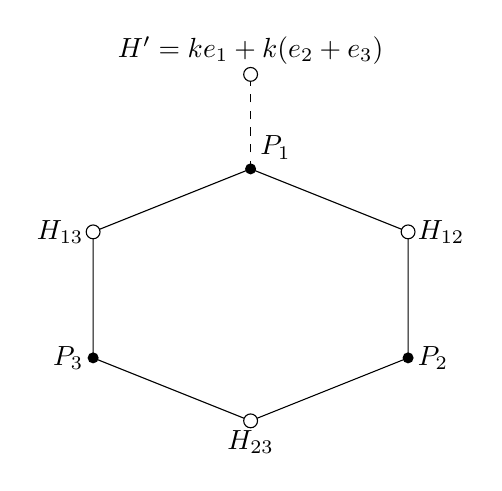
\begin{tikzpicture}
		\coordinate (P1) at (0,1.6);
		\coordinate (H12) at (2,0.8);
		\coordinate (P2) at (2,-0.8);
		\coordinate (H23) at (0,-1.6);
		\coordinate (P3) at (-2,-0.8);
		\coordinate (H13) at (-2,0.8);
		\coordinate (Hp) at (0,2.8);
		\draw (P1)--(H12)--(P2)--(H23)--(P3)--(H13)--cycle;
		\draw[dashed] (P1)--(Hp);
		\foreach \p in {P1,P2,P3} {\fill (\p) circle (2pt);}
		\foreach \h in {H12,H23,H13,Hp} {\draw[fill=white] (\h) circle (2.5pt);}
		\node[above right] at (P1) {\(P_1\)};
		\node[right] at (H12) {\(H_{12}\)};
		\node[right] at (P2) {\(P_2\)};
		\node[below] at (H23) {\(H_{23}\)};
		\node[left] at (P3) {\(P_3\)};
		\node[left] at (H13) {\(H_{13}\)};
		\node[above] at (Hp) {\(H'=ke_1+k(e_2+e_3)\)};
	\end{tikzpicture}
	\caption[\(A_2\) 型坐标公寓]{\(A_2\) 型坐标公寓。实心点表示一维子空间，空心点表示二维子空间；实线六边形是一个公寓，虚线是一条离开该公寓的旗。}
	\label{b5:fig:F-A2-apartment}
\end{figure}

这些公寓彼此重叠。要使它们能够一致地描述不同位置的旗，除了每个公寓具有相同模型以外，还需要两条相容条件。

\begin{definition}\label{b5:def:F-A-building}
	设 \(n\ge2\)，\(\Delta\) 为一个单纯复形，其顶点带有 \(1,\ldots,n-1\) 中的型，每个单纯形的顶点型互不相同。给定一族子复形 \(\mathscr A\)，其中每个成员都保型同构于 \(A_{n-1}\) 型的上述子集链复形。若满足以下条件，则称 \((\Delta,\mathscr A)\) 为一个 \(A_{n-1}\) 型的\term[lou]{球面楼}[spherical building]，其秩为 \(n-1\)：
	\begin{enumerate}
		\item 任意两个单纯形都包含于某个公寓中。
		\item 对任意两个公寓 \(\mathcal A,\mathcal A'\)，存在保型的复形同构 \(\mathcal A\to\mathcal A'\)，使两者交集中每个顶点保持不变。
	\end{enumerate}
	这里复形同构是顶点集合的双射，要求它和它的逆都把单纯形送到单纯形；保型是指不改变顶点的型。
\end{definition}

定义中的秩是室的顶点数；相应复形的维数比秩少 \(1\)。本节只使用这一 \(A\) 型模型。一般球面楼以其他有限 Coxeter 群的复形取代子集链复形；其公寓公理及与 BN 对的关系可参看\cite[Chapter 9, pp. 97--100]{Taylor1992ClassicalGroups}。

\begin{theorem}\label{b5:thm:F-vector-building}
	设 \(V\) 为域 \(k\) 上的 \(n\) 维向量空间，\(n\ge2\)。旗复形 \(\Delta(V)\) 连同所有坐标公寓构成一个 \(A_{n-1}\) 型球面楼。
\end{theorem}

\begin{proof}
	每个坐标公寓已经由 \(I\mapsto V_I\) 与子集链模型保型同构。给定两个单纯形，由\cref{b5:prop:F-chambers-flags}把它们分别补成完全旗。\cref{b5:lem:F-common-flag-basis}给出同时适配这两面完全旗的一组基，因此两面旗和原来的两个单纯形均包含于该基的坐标公寓。这证明第一条公理。

	第二条公理要求同时固定所有共有子空间，而不只是选择一面共有旗。设两个公寓分别由基 \((e_1,\ldots,e_n)\)、\((f_1,\ldots,f_n)\) 给出，写
	\[
		f_j=\sum_{i=1}^n a_{ij}e_i,
		\qquad A=(a_{ij})\in\operatorname{GL}_n(k).
	\]
	由于 \(\det A\ne0\)，其行列式展开中至少有一项非零，所以可以选择 \(\sigma\in S_n\)，使 \(a_{\sigma(j),j}\ne0\) 对每个 \(j\) 都成立。由 \(f_j\mapsto e_{\sigma(j)}\) 定义线性同构 \(T:V\to V\)。它把 \(f\) 基的坐标子空间送到 \(e\) 基的坐标子空间，因而给出公寓之间的保型复形同构。

	设 \(U\) 是这两个公寓共有的顶点。存在唯一指标集 \(I,J\)，使
	\[
		U=\operatorname{span}_k\{\,e_i\mid i\in I\,\}
		 =\operatorname{span}_k\{\,f_j\mid j\in J\,\}.
	\]
	若 \(j\in J\)，则 \(f_j\in U\)，故 \(a_{ij}=0\) 对每个 \(i\notin I\) 成立。选出的非零项迫使 \(\sigma(j)\in I\)，于是 \(\sigma(J)\subseteq I\)。又 \(\lvert I\rvert=\dim U=\lvert J\rvert\)，从而 \(\sigma(J)=I\)，即 \(T(U)=U\)。同一个 \(T\) 对每个共有顶点都满足这一等式，因此它在公寓交集上固定全部顶点。取其逆即得定义所需方向的同构。这里固定的是作为顶点的子空间，不要求 \(T\) 固定该子空间中的每个向量。
\end{proof}

上述证明把“两旗有共同适配基”与“两个坐标模型能在交集上相合”分开处理。前者控制两室的相对位置，后者保证换公寓时共同的面仍表示同一个子空间。有限域只在计数时才是必要条件，楼的这项线性代数构造对任意域都成立。

\subsection{公寓、室与余维一邻接}
\label{b5:subsec:F03:03}

在一个坐标公寓中，固定除 \(i\) 维子空间以外的全部旗项，补回这一项只有两种坐标选择；在整个旗复形中却有更多选择。这个差别可以在一个二维商空间内完全算清。

\begin{proposition}\label{b5:prop:F-panel-count}
	设 \(V\) 为 \(\mathbb F_q\) 上的 \(n\) 维向量空间，\(n\ge2\)。\(\Delta(V)\) 的每个余维一面恰包含于 \(q+1\) 个室中；若该面位于一个固定公寓，则其中恰有两个室属于该公寓。因此，每个室对每种型 \(i\in\{1,\ldots,n-1\}\) 恰有 \(q\) 个不同的 \(i\)-相邻室，总共有 \((n-1)q\) 个相邻室。
\end{proposition}

\begin{proof}
	设给定的余维一面缺少型 \(i\)。把端点补成 \(V_0=0,V_n=V\)，其两侧已给定的子空间是 \(V_{i-1}<V_{i+1}\)。补回一室等价于选择
	\[
		V_{i-1}<W<V_{i+1},\qquad \dim W=i.
	\]
	映射 \(W\mapsto W/V_{i-1}\) 将这些选择与二维空间 \(V_{i+1}/V_{i-1}\) 中的一维子空间一一对应，逆映射是取商映射下的原像。后一集合有 \((q^2-1)/(q-1)=q+1\) 个元素。

	若余维一面位于一个固定坐标公寓，则代表 \(V_{i+1}\) 的坐标指标集比代表 \(V_{i-1}\) 的指标集恰多两个指标。在公寓内补回 \(W\)，只能先加入其中一个指标，故恰有两个选择。固定一个室后，其中一个选择是原室；在整个楼内，其余 \(q\) 个选择才是不同的相邻室。不同型的相邻室改变的是不同维数的旗项，不会重复计算，所以总数为 \((n-1)q\)。
\end{proof}

每个余维一面恰含于两个室的复形称为\term[bao-fuxing]{薄复形}[thin complex]；若每个余维一面至少含于三个室，则称为\term[hou-fuxing]{厚复形}[thick complex]。所以公寓是薄的，而 \(\Delta(\mathbb F_q^n)\) 是厚的。\cref{b5:fig:F-A2-apartment}中 \(P_1\) 在公寓内只连着 \(H_{12},H_{13}\)，但整个楼至少还有 \(H'\) 这一选择。当 \(q=2\) 时，三个选择恰好全部画出。

\ProseParagraphBreak

公寓的室用排列 \(w\) 编号时，\(i\)-相邻恰好交换排列列表中第 \(i\)、\(i+1\) 两项，即把 \(w\) 换成 \(ws_i\)，其中 \(s_i=(i\ i+1)\)。这是因为只交换这两个指标，会且只会改变由前 \(i\) 个基向量张成的子空间。任意排列都可由相邻换位得到，所以公寓内任意两室可以经有限次余维一邻接相连。任意两室又同处某个公寓，故整个旗复形的室也具有这一连通性。\(A_2\) 公寓的六个室依次围成一圈，从一室到对面一室的两条三步路径分别具有型序列 \((1,2,1)\) 与 \((2,1,2)\)，对应于 \(s_1s_2s_1=s_2s_1s_2\)。

\ProseParagraphBreak

这里有两张应当区别的图。三维时，旗复形本身的顶点是射影点和射影直线，室是它的边；若另外把室作为顶点、把余维一邻接作为边，就得到室的邻接图。固定一个余维一面的 \(q+1\) 个室在后一张图中两两相邻，所以会出现三角形；这不表示原来的点线关联图中也出现了三角形。后一种邻接将用于下一节定义旗上的算子，而其中的参数 \(q\) 正是每个给定型的不同相邻室数。

% !TeX root = ../../Book5.tex
% 纲要标题：### F.4 阶、Sylow 子群与 Hecke 代数
% 纲要位置：工作记录/计划纲要.md（2026-10-20 新增骨架）。
% 写作状态：2026-10-20 新增骨架；正文、证明、算例与习题均待撰写。
% 写作范围：以经典群、旗与小秩计算为范围，不展开一般群概形构造、楼的完整理论及 Deligne–Lusztig 理论。
% #### F.4.1 经典群的阶与 Sylow 子群
% #### F.4.2 旗上的相容算子与 Hecke 代数
% #### F.4.3 小秩计算与证明范围

\section{阶、Sylow 子群与 Hecke 代数}
\label{b5:sec:F04}

待撰写。

\subsection{经典群的阶与 Sylow 子群}
\label{b5:subsec:F04:01}

待撰写。

\subsection{旗上的相容算子与 Hecke 代数}
\label{b5:subsec:F04:02}

待撰写。

\subsection{小秩计算与证明范围}
\label{b5:subsec:F04:03}

待撰写。

% 新增结构与纲要同步；以下条目均为待撰写计划。
% * 状态：待撰写；当前仅有结构占位。
% ---


\begin{chaptersummary}
	有限域上的矩阵关系给出经典群，Frobenius 不动点则说明它们如何从代数闭包上的群恢复。根子群沿一个参数作加法，交换子把不同根方向联系起来；群的阶还需要对整个空间的基或辛基计数。定义特征的 Sylow 子群可以由这些单位三角矩阵直接构造，其他素数的 Sylow 子群未必具有同样的形状。
	\ProseParagraphBreak
	两个完全旗的交维数确定一个置换，由此得到 Bruhat 分解、BN 对与抛物双陪集。把旗组成复形后，坐标基给出公寓，而余维一面上的 \(q+1\) 个室控制邻接计数。相对位置算子的乘法因此出现 \(q\) 和 \(q-1\)，与抽象 Hecke 代数的二次关系一致。群阶、旗数与相容算子代数的维数分别记录不同信息；低秩中的表示分解还取决于表示系数域的特征。
\end{chaptersummary}

\BookExercises

\begin{exercise}\label{b5:ex:F-projective-determinant}
	设 \(q\) 为素数幂，\(n\ge2\)。证明矩阵的行列式诱导满同态
	\[
		\operatorname{PGL}_n(q)\longrightarrow
		\mathbb F_q^\times/(\mathbb F_q^\times)^n,
	\]
	其核为 \(\operatorname{PSL}_n(q)\) 的自然像。求 \([\operatorname{PGL}_n(q):\operatorname{PSL}_n(q)]\)，并判断哪些 \(n,q\) 使每个可逆矩阵的射影类都有行列式一的代表。以 \(n=2,q=3\) 写出一个没有这种代表的具体射影类。
\end{exercise}
\begin{solution}
	同一射影类的两个代表为 \(g\) 与 \(ag\)，其中 \(a\in\mathbb F_q^\times\)。其行列式相差因子 \(a^n\)，所以行列式在所给商群中的类与代表无关。它保持乘法，并因 \(\operatorname{diag}(b,1,\ldots,1)\) 实现每个非零行列式而满射。

	若 \(\det g=a^n\)，则 \(a^{-1}g\) 的行列式为一；反过来，射影类若有这样的代表，其行列式的类必为单位。所以核恰为特殊线性群的射影像。\(\operatorname{SL}_n(q)\) 到 \(\operatorname{PGL}_n(q)\) 的核为 \(a^n=1\) 的标量，故其像确实同构于定义中的 \(\operatorname{PSL}_n(q)\)。

	乘法群 \(\mathbb F_q^\times\) 是 \(q-1\) 阶循环群，取 \(n\) 次幂的像有 \((q-1)/\gcd(n,q-1)\) 个元素。因此所求指数为 \(\gcd(n,q-1)\)，每个射影类都有行列式一代表当且仅当这个最大公因数为一。在 \(\mathbb F_3\) 上，\(g=\operatorname{diag}(1,-1)\) 的行列式为 \(-1\)，而每个非零标量的平方都为一，故任何标量倍的行列式仍为 \(-1\)。
\end{solution}

\begin{exercise}\label{b5:ex:F-quadratic-two-forms}
	在 \(V=\mathbb F_2^2\) 上取 \(Q_0(x,y)=xy\) 与 \(Q_1(x,y)=x^2+xy+y^2\)。证明两型有相同的非退化极化型，求它们的正交群，并说明为何 \(\operatorname O(V,Q_0)\) 是该极化型的辛群的真子群，而 \(\operatorname O(V,Q_1)\) 恰为该辛群。
\end{exercise}
\begin{solution}
	平方项在特征二中的极化为零，故两型的极化型都是
	\[
		b\bigl((x,y),(x',y')\bigr)=xy'+x'y,
	\]
	其矩阵 \(\bigl(\begin{smallmatrix}0&1\\1&0\end{smallmatrix}\bigr)\) 可逆。三个非零向量是 \(e_1,e_2,e_1+e_2\)。\(Q_0\) 仅在前两个非零向量上为零，所以保持 \(Q_0\) 的可逆变换必须保持集合 \(\{e_1,e_2\}\)，只有恒等与交换这两个基向量两种，故 \(\operatorname O(V,Q_0)\cong C_2\)。

	\(Q_1\) 在三个非零向量上均为一，因而每个可逆线性变换都保持 \(Q_1\)。\(\operatorname{GL}_2(2)\) 对这三个向量的作用忠实：若全部固定，则尤其固定一组基。它又有 \((4-1)(4-2)=6\) 个元素，所以这个作用给出 \(\operatorname{GL}_2(2)\cong S_3\)。另一方面，对任意二阶矩阵 \(g\)，直接计算得到 \(g^{\mathsf T}J_1g=(\det g)J_1\)，而 \(\mathbb F_2^\times=\{1\}\)，所以 \(\operatorname{Sp}_2(2)=\operatorname{GL}_2(2)\)。于是 \(\operatorname O(V,Q_1)\cong S_3\)，而 \(\operatorname O(V,Q_0)\) 是其中的二阶真子群。相同的极化型在这里对应两个不同的正交群。
\end{solution}

\begin{exercise}\label{b5:ex:F-unitary-isotropic-root}
	设 \(q=p^r\)，在 \(V=\mathbb F_{q^2}^2\) 上取 \(h(v,w)=\bar v^{\mathsf T}w\)、\(\bar a=a^q\)。
	\begin{enumerate}
		\item 证明满足 \(h(v,v)=0\) 的一维子空间恰有 \(q+1\) 条。
		\item 固定一个满足 \(h(v,v)=0\) 的非零向量 \(v\)。对 \(a\in\mathbb F_{q^2}\)，令 \(T_a(w)=w+a\,h(v,w)v\)。证明 \(T_a\in\operatorname{SU}_2(q)\) 当且仅当 \(a+\bar a=0\)。
		\item 证明这批 \(T_a\) 组成一个 \(q\) 阶子群，其每个非单位元素的阶为 \(p\)。
	\end{enumerate}
\end{exercise}
\begin{solution}
	1. 各向同性向量 \((x,y)\ne0\) 必有 \(y\ne0\)，否则 \(x^{q+1}=0\) 使 \(x=0\)。每条这样的直线因而有唯一代表 \((t,1)\)，条件为 \(t^{q+1}=-1\)。正文已经说明范数 \(\mathbb F_{q^2}^\times\to\mathbb F_q^\times\) 满射且核有 \(q+1\) 个元素，所以 \(-1\) 的原像恰有 \(q+1\) 个元素。

	2. 令 \(N(w)=h(v,w)v\)。它是 \(\mathbb F_{q^2}\) 线性映射，满足 \(N^2=0\)，所以 \(T_a=I+aN\) 可逆。\(N\) 杀掉 \(v\)，并把整个空间映入 \(\mathbb F_{q^2}v\)；以 \(v\) 为首向量补成基，\(T_a\) 的矩阵是对角项都为一的上三角矩阵，故其行列式为一。计算型的变化得到
	\[
		h(T_aw,T_az)-h(w,z)
		=(a+\bar a)h(w,v)h(v,z).
	\]
	这里二次项因 \(h(v,v)=0\) 消失，两个一次项使用 \(\overline{h(v,w)}=h(w,v)\)。若 \(a+\bar a=0\)，型得到保持。反过来，由 \(h\) 非退化且 \(v\ne0\)，可取 \(w,z\) 使 \(h(w,v)\)、\(h(v,z)\) 都非零；若型保持，上式就迫使 \(a+\bar a=0\)。

	3. 映射 \(a\mapsto a+\bar a\) 从二维 \(\mathbb F_q\) 空间 \(\mathbb F_{q^2}\) 线性映到 \(\mathbb F_q\)。它不是零映射：若 \(p\ne2\)，一的像是二；若 \(p=2\) 而它恒为零，就有 \(a^q=a\) 对全部 \(a\) 成立，与 \(X^q-X\) 只有 \(q\) 个根矛盾。故它满射，核是一维 \(\mathbb F_q\) 空间，有 \(q\) 个元素。由 \(N^2=0\)，\(T_aT_b=T_{a+b}\)；又因 \(N\ne0\)，参数映射单射。因此这个子群同构于 \((\mathbb F_q,+)\)，结论随之成立。
\end{solution}

\begin{exercise}\label{b5:ex:F-upper-three-exponent}
	设 \(q=p^r\)，令 \(U\) 为全部矩阵
	\[
		u(a,b,c)=\begin{pmatrix}1&a&c\\0&1&b\\0&0&1\end{pmatrix},\qquad a,b,c\in\mathbb F_q
	\]
	组成的群。求其中心与交换子子群，并计算任意 \(u(a,b,c)^s\)、\(s\ge0\)。由此证明：\(p\) 为奇数时，\(U\) 的指数为 \(p\)；\(p=2\) 时，\(U\) 的指数为四。解释为什么后一结论不与根子群中非单位元素的阶为二矛盾。
\end{exercise}
\begin{solution}
	由正文的乘法公式，逆为 \(u(a,b,c)^{-1}=u(-a,-b,ab-c)\)，并且
	\[
		[u(a,b,c),u(a',b',c')]=u(0,0,ab'-a'b).
	\]
	这个交换子对全部 \(a',b'\) 恒为单位，当且仅当 \(a=b=0\)：先取 \(a'=0,b'=1\) 得 \(a=0\)，再取 \(a'=1,b'=0\) 得 \(b=0\)。所以 \(Z(U)=\{\,u(0,0,c)\mid c\in\mathbb F_q\,\}\)。所有交换子落在这里，而取 \(a=1,b'=c,a'=b=0\) 又实现任意 \(u(0,0,c)\)，故 \([U,U]=Z(U)\)。

	对 \(s\) 用乘法公式归纳，得到
	\[
		u(a,b,c)^s=u\left(sa,sb,sc+\binom{s}{2}ab\right),
	\]
	其中整数系数按特征 \(p\) 映入域中。若 \(p\) 为奇数，\(p\mid\binom p2\)，故每个元素的 \(p\) 次幂为单位，而 \(u(1,0,0)\) 的阶为 \(p\)，所以指数恰为 \(p\)。若 \(p=2\)，则 \(u(a,b,c)^2=u(0,0,ab)\)，再平方为单位；取 \(a=b=1,c=0\)，其平方非单位，所以指数为四。根子群中的矩阵各自只有一个非对角参数；它们的乘积可同时含有两个相邻方向，平方产生新的 \((1,3)\) 条目，因而不必仍有二阶。
\end{solution}

\begin{exercise}\label{b5:ex:F-Grassmann-orbit-size}
	设 \(q\) 为素数幂，\(V=\mathbb F_q^n\)，\(0\le k,l\le n\)，固定一个 \(k\) 维子空间 \(U\)。对满足 \(\max(0,k+l-n)\le r\le\min(k,l)\) 的整数 \(r\)，求全部满足 \(\dim W=l\)、\(\dim(U\cap W)=r\) 的子空间 \(W\) 的数目，并由此证明
	\[
		{n\brack l}_q=
		\sum_r q^{(k-r)(l-r)}{k\brack r}_q{n-k\brack l-r}_q.
	\]
	这里 \({a\brack b}_q\) 是 \(\mathbb F_q^a\) 的 \(b\) 维子空间数。
\end{exercise}
\begin{solution}
	先选 \(R=U\cap W\)，有 \({k\brack r}_q\) 种选择。商映射 \(\pi:V\to V/U\) 将 \(W\) 送到一个 \(l-r\) 维子空间 \(L\)，共有 \({n-k\brack l-r}_q\) 种选择。固定 \(R,L\) 后，在 \(\pi^{-1}(L)/R\) 中，\(W/R\) 必须与 \(U/R\) 互补。选一次线性分裂，把此空间写成 \((U/R)\oplus L\)；每个这样的补空间唯一为某个线性映射 \(f:L\to U/R\) 的图。反过来，每个图都给出一个所求的 \(W\)。因此固定 \(R,L\) 后有 \(q^{(k-r)(l-r)}\) 种选择，总数为
	\[
		q^{(k-r)(l-r)}{k\brack r}_q{n-k\brack l-r}_q.
	\]
	所有 \(l\) 维子空间按 \(r=\dim(U\cap W)\) 不交分组，求和即得恒等式。例如 \(n=4,k=l=2,r=0\) 时，有 \(q^4\) 个与 \(U\) 互补的二维子空间；\(r=1\) 时则有 \(q(q+1)^2\) 个。
\end{solution}

\begin{exercise}\label{b5:ex:F-SL-BN}
	设 \(G_0=\mathrm{SL}_n(\mathbb F_q)\)，\(n\ge2\)，\(B_0,N_0\) 分别为其中的上三角矩阵子群与单项矩阵子群。证明它们给出 Weyl 群为 \(S_n\) 的 BN 对，并且每个 Bruhat 旗轨道仍含 \(q^{\ell(w)}\) 个旗。说明为什么在奇特征时，不能把所有普通置换矩阵直接用作 \(G_0\) 中的提升。
\end{exercise}
\begin{solution}
	任意置换矩阵 \(n_w\) 都可左乘一个对角矩阵，使所得 \(\widetilde n_w\) 的行列式为一。此调整不改变对坐标直线的置换，故 \(N_0\to S_n\) 满射，核为 \(T_0=B_0\cap N_0\)，即行列式为一的对角子群。任意完全旗可写为 \(gE\)，\(g\in\mathrm{GL}_n(\mathbb F_q)\)；右乘一个行列式为 \((\det g)^{-1}\) 的对角矩阵不改变旗，因此 \(G_0\) 对全部完全旗仍传递作用，稳定子群为 \(B_0\)。

	\(B_0\) 与 \(B\) 在完全旗集上的轨道相同。为看出这一点，固定 \(w\)，注意全部对角矩阵既固定标准旗，也固定 \(n_wE\)。对 \(b\in B\)，取对角矩阵 \(t\) 使 \(\det t=(\det b)^{-1}\)，就有 \(bt\in B_0\) 且 \(bt n_wE=bn_wE\)。所以 \(B_0\) 的轨道仍由 \(w\) 标记，且大小不变。由旗轨道读出
	\[
		G_0=\bigsqcup_{w\in S_n}B_0\widetilde n_wB_0,
	\]
	从而 \(G_0=\langle B_0,N_0\rangle\)。\(i\) 型相邻旗仍有 \(q\) 个，\cref{b5:prop:F-flag-adjacency}只涉及旗与二维商，不涉及矩阵行列式；因此同一个论证给出 BN 乘法公理。

	可取简单反射提升在第 \(i,i+1\) 个坐标上的矩阵块为 \(\begin{psmallmatrix}0&-1\\1&0\end{psmallmatrix}\)，在其余坐标上为单位。它把上三角根元素 \(I_n+E_{i,i+1}\) 共轭到 \(I_n-E_{i+1,i}\)，后者不在 \(B_0\)，即使特征为二也仍如此。非退化公理亦成立。普通置换矩阵的行列式为置换符号，在奇特征时，奇置换的矩阵不属于 \(\mathrm{SL}_n\)；上述对角修正不能省略。
\end{solution}

\begin{exercise}\label{b5:ex:F-parabolic-normalizer}
	设 \(G=\mathrm{GL}_n(\mathbb F_q)\)，\(B\) 为可逆上三角子群。证明 \(B\) 的不变子空间恰为标准旗中的 \(E_0,E_1,\ldots,E_n\)。进而求标准抛物子群 \(P_I\) 的全部不变子空间，并证明 \(N_G(P_I)=P_I\)。
\end{exercise}
\begin{solution}
	若 \(0\ne W\le V\) 被 \(B\) 保持，取所有 \(W\) 中向量出现的非零坐标的最大指标 \(r\)，则 \(W\subseteq E_r\)，且存在 \(v\in W\) 的第 \(r\) 个坐标 \(v_r\ne0\)。对每个 \(i<r\)，矩阵 \(I_n+E_{ir}\) 属于 \(B\)，所以
	\[
		(I_n+E_{ir})v-v=v_r e_i\in W.
	\]
	由此 \(e_1,\ldots,e_{r-1}\in W\)；再从 \(v\) 减去其前 \(r-1\) 个坐标部分，得到 \(v_r e_r\in W\)。因此 \(W=E_r\)。反过来，上三角矩阵保持每个 \(E_r\)，故列出的确是全部。

	因为 \(B\subseteq P_I\)，任何 \(P_I\) 不变子空间也必为某个 \(E_r\)。当 \(1\le r<n\) 时，\(E_r\) 被所有 \(n_s\)、\(s\in I\)，保持，当且仅当 \(s_r\notin I\)：只有交换第 \(r,r+1\) 个坐标会破坏 \(E_r\)。故全部不变子空间正是定义 \(P_I\) 的标准部分旗，加上 \(0,V\)。

	若 \(g\in N_G(P_I)\)，则 \(g\) 将一个 \(P_I\) 不变子空间送到另一个同维的不变子空间。每个保留维数只有一个这样的子空间，因而 \(g\) 固定定义 \(P_I\) 的部分旗。由\cref{b5:prop:F-parabolic-flags}，\(g\in P_I\)。反向包含显然成立，所以 \(P_I\) 自正规化。
\end{solution}

\begin{exercise}\label{b5:ex:F-BN-product}
	设 \((B,N)\) 为群 \(G\) 的 BN 对，\(H\) 为任意群。证明 \((B\times H,N\times H)\) 为 \(G\times H\) 的 BN 对，且 Weyl 群与简单反射集不变。由此说明，抽象 BN 对的公理本身并不要求 \(B\) 是可解群。
\end{exercise}
\begin{solution}
	新交集为 \((B\cap N)\times H\)，在 \(N\times H\) 中正规，其商自然同构于 \(N/(B\cap N)\)。可取提升 \((n_w,1)\)。生成条件由 \(G=\langle B,N\rangle\) 及 \(1\times H\subseteq B\times H\) 得到。BN 乘法公理两边分别是原相应集合与 \(H\) 的直积，所以原包含关系给出新包含关系。共轭 \((n_s,1)(B\times H)(n_s,1)^{-1}\) 等于 \((n_sBn_s^{-1})\times H\)，仍不包含于 \(B\times H\)。因此全部公理成立。

	例如取已建立的 \(\mathrm{GL}_2(\mathbb F_2)\) 的 BN 对，并取 \(H=A_5\)。新子群 \(B\times A_5\) 有非可解商群 \(A_5\)，所以不可解。这并不影响它满足 BN 对的公理，说明具体上三角群的性质不能未经证明推广到任意 BN 对。
\end{solution}

\begin{exercise}\label{b5:ex:F-projective-plane-graph}
	令 \(\Gamma\) 为 \(\Delta(\mathbb F_q^3)\) 的点线关联图。求两类顶点数、每个顶点的度数及边数；证明它的最短简单回路长为 \(6\)，任意两顶点之间的最大距离为 \(3\)。
\end{exercise}
\begin{solution}
	一维子空间数为 \((q^3-1)/(q-1)=q^2+q+1\)。每个二维子空间都是一个非零线性泛函的核，而两个非零泛函的核相同当且仅当它们相差一个非零倍数，故二维子空间数也为 \(q^2+q+1\)。给定一维子空间 \(P\)，包含它的二维子空间与二维商空间 \(\mathbb F_q^3/P\) 中的一维子空间对应，因而有 \(q+1\) 个。每个二维子空间中也有 \(q+1\) 个一维子空间。所以每个顶点的度数为 \(q+1\)，边数为 \((q^2+q+1)(q+1)\)；数边时只从一类顶点出发，不再乘 \(2\)。例如 \(q=2\) 时共有 \(14\) 个顶点和 \(21\) 条边。

	这是一张没有重边的二部图，因此简单回路的长度至少为 \(4\) 且为偶数。若存在四边形，则其两个不同射影点同时落在两个不同射影直线上。但两个不同的一维子空间张成唯一的二维子空间，矛盾。一组基给出的公寓则确实是一条六边形，所以最短简单回路长为 \(6\)。

	两个不同射影点经它们张成的射影直线相连，距离为 \(2\)；两个不同射影直线经其一维交相连，距离也为 \(2\)。点 \(P\) 与直线 \(H\) 若关联，距离为 \(1\)。若不关联，取 \(P'\subset H\) 为任意射影点，再令 \(H'=P+P'\)，便有长度为 \(3\) 的路径 \(P-H'-P'-H\)。二部性排除长度为 \(2\) 的路径，不关联又排除长度 \(1\)，故此时距离恰为 \(3\)。存在不关联点线，例如 \(\mathbb F_q e_1\) 与 \(\mathbb F_q e_2+\mathbb F_q e_3\)，所以最大距离确为 \(3\)。
\end{solution}

\begin{exercise}\label{b5:ex:F-apartment-count}
	设 \(V=\mathbb F_q^n\)，\(n\ge2\)。证明其旗复形中的不同坐标公寓数为
	\[
		\frac{|\operatorname{GL}_n(\mathbb F_q)|}{n!(q-1)^n},
	\]
	并证明每个室恰属于 \(q^{n(n-1)/2}\) 个公寓。解释为何换用另一组基，不一定得到另一个公寓。
\end{exercise}
\begin{solution}
	有序基的数量为 \(|\operatorname{GL}_n(\mathbb F_q)|\)。一个公寓的一维顶点恰好是生成它的 \(n\) 条坐标直线，所以公寓唯一决定这组无序直线。反过来，在每条直线上选择一个非零向量，再给这些向量排序，便得到产生同一公寓的全部有序基，共有 \((q-1)^n n!\) 组。因此不同公寓数为所给商式。这里能直接除，是因为每个公寓对应的基数完全相同；对基向量分别作非零倍乘或重新排序都不改变公寓。

	固定一个室 \(C\)。\(\operatorname{GL}_n(\mathbb F_q)\) 在室上作用传递，故每个室属于同样多的公寓，记此数为 \(a\)。室的稳定子是可逆上三角矩阵群，其阶为 \((q-1)^nq^{n(n-1)/2}\)，所以室数为
	\[
		\frac{|\operatorname{GL}_n(\mathbb F_q)|}{(q-1)^nq^{n(n-1)/2}}.
	\]
	每个公寓含有 \(n!\) 个室。按两种次序计算满足 \(C\subset\mathcal A\) 的对 \((C,\mathcal A)\)，得到
	\[
		a\,\frac{|\operatorname{GL}_n(\mathbb F_q)|}{(q-1)^nq^{n(n-1)/2}}
		=\frac{|\operatorname{GL}_n(\mathbb F_q)|}{n!(q-1)^n}\,n!.
	\]
	约去非零因子便得 \(a=q^{n(n-1)/2}\)。例如 \(\mathbb F_2^3\) 的旗复形有 \(28\) 个公寓，每室属于 \(8\) 个公寓。
\end{solution}

\begin{exercise}\label{b5:ex:F-flag-link}
	设 \(V=\mathbb F_q^4\)，固定二维子空间 \(U\)。定义 \(U\) 在旗复形中的链环为
	\[
		\operatorname{link}_{\Delta(V)}(U)
		=\{\,\sigma\in\Delta(V)\mid U\notin\sigma,\ \sigma\cup\{U\}\in\Delta(V)\,\}.
	\]
	证明这个链环是一张完全二部图 \(K_{q+1,q+1}\)，并求包含 \(U\) 的室数。若再固定一个包含 \(U\) 的坐标公寓，证明其内部的对应链环是四边形。
\end{exercise}
\begin{solution}
	能与 \(U\) 同在一条旗中的其他顶点，只能是 \(U\) 中的一维子空间 \(L\)，或包含 \(U\) 的三维子空间 \(H\)。第一类有 \(q+1\) 个；第二类经 \(H\mapsto H/U\) 与二维空间 \(V/U\) 中的一维子空间对应，也有 \(q+1\) 个。任意一对这样的 \(L,H\) 都满足 \(L<U<H\)，所以链环中每个第一类顶点都连向每个第二类顶点；同类的两个顶点维数相等，不可能同时属于一条旗，因此不相连。链环恰为 \(K_{q+1,q+1}\)。其边与含 \(U\) 的完全旗一一对应，所以这样的室共有 \((q+1)^2\) 个。

	在一个包含 \(U\) 的坐标公寓中，重新排列基后可写 \(U=\mathbb F_q e_1+\mathbb F_q e_2\)。公寓内小于 \(U\) 的一维顶点只有 \(\mathbb F_q e_1,\mathbb F_q e_2\)，大于 \(U\) 的三维顶点只有 \(U+\mathbb F_q e_3,U+\mathbb F_q e_4\)。四种包含组合都成立，所以对应链环为 \(K_{2,2}\)，即四边形。这与三维空间中公寓的六边形不同：固定中间的二维子空间以后，\(U\) 内的一维选择和 \(V/U\) 内的一维选择彼此独立。
\end{solution}

\begin{exercise}\label{b5:ex:F-building-duality}
	设 \(V=k^n\)，\(n\ge3\)，在 \(V\) 上取标准非退化对称双线性型 \(\beta(x,y)=\sum_i x_i y_i\)。对每个子空间 \(U\) 记
	\[
		U^\perp=\{\,v\in V\mid\beta(v,u)=0\;\text{对所有}\;u\in U\,\}.
	\]
	证明 \(U\mapsto U^\perp\) 在旗复形 \(\Delta(V)\) 上诱导一个对合自同构，但它不保持顶点的型，也不是由 \(\operatorname{GL}(V)\) 中的元素给出的。证明它把坐标公寓送到坐标公寓，并说明 \(n=3\) 时对点线关联图的作用。
\end{exercise}
\begin{solution}
	非退化性使 \(V\to V^*\)、\(v\mapsto\beta(v,-)\) 为同构。复合限制满射 \(V^*\to U^*\)，得到核为 \(U^\perp\) 的满射 \(V\to U^*\)。所以 \(\dim U^\perp=n-\dim U\)。对称性给出 \(U\subseteq(U^\perp)^\perp\)，两边维数相同，故 \((U^\perp)^\perp=U\)。此外，\(U\subseteq W\) 蕴涵 \(W^\perp\subseteq U^\perp\)。因此一条非零真子空间链经过取正交补并反转排列后仍是一条链；再次取正交补恢复原链，从而得到复形的对合自同构。

	它把型 \(i\) 换成型 \(n-i\)。因 \(n\ge3\)，一维顶点变成 \((n-1)\) 维顶点，故不保型；线性同构总保持维数，所以这个自同构不来自 \(\operatorname{GL}(V)\)。复形自同构与楼定义中要求的保型同构由此需要区分。

	若 \(e_1,\ldots,e_n\) 是任意基，由非退化性存在唯一的 \(\beta\)-对偶基 \(f_1,\ldots,f_n\)，满足 \(\beta(f_i,e_j)=\delta_{ij}\)。对每个指标集 \(I\)，
	\[
		\bigl(\operatorname{span}_k\{\,e_i\mid i\in I\,\}\bigr)^\perp
		=\operatorname{span}_k\{\,f_j\mid j\notin I\,\}.
	\]
	所以 \(e\) 基公寓被送到 \(f\) 基公寓。三维时，该映射交换射影点与射影直线；若 \(P\subset H\)，则 \(H^\perp\subset P^\perp\)，因此点线关联仍被保持，但两类顶点互换。
\end{solution}

\begin{exercise}\label{b5:ex:F-nondefining-sylow}
	在 \(G=\operatorname{GL}_2(\mathbb F_5)\) 中取
	\[
		A=\begin{pmatrix}0&-1\\1&-1\end{pmatrix},\qquad
		U=\left\{\,\begin{pmatrix}1&a\\0&1\end{pmatrix}:a\in\mathbb F_5\,\right\}.
	\]
	证明 \(\langle A\rangle\) 与 \(U\) 分别为 Sylow 三子群与 Sylow 五子群，并证明 \(\langle A\rangle\) 不保持任何 \(\mathbb F_5\) 直线。因此，它不能通过 \(G\) 中的共轭变成上三角子群。
\end{exercise}
\begin{solution}
	群阶为 \((25-1)(25-5)=480=2^5\cdot3\cdot5\)。直接相乘有 \(A^2+A+I=0\)，从而 \(A^3=I\)，而 \(A\ne I\)，故 \(\langle A\rangle\) 的阶为三。\(U\) 与 \((\mathbb F_5,+)\) 同构，阶为五。它们分别实现群阶中的最大 \(3\) 幂与 \(5\) 幂因子，因而都是所称的 Sylow 子群。

	若某条 \(\mathbb F_5\) 直线被 \(A\) 保持，其上有非零向量 \(v\) 满足 \(Av=av\)、\(a\in\mathbb F_5\)，于是 \(a^2+a+1=0\)。但这个二次式的判别式为 \(-3=2\)，不是 \(\mathbb F_5\) 中的平方，故无根。上三角子群保持第一条坐标直线；若某个共轭将 \(\langle A\rangle\) 放进该子群，拉回这条直线就得到 \(\langle A\rangle\) 的不变直线，矛盾。定义特征和非定义特征的 Sylow 子群在这里已有不同的旗作用。
\end{solution}

\begin{exercise}\label{b5:ex:F-symplectic-sylow-four}
	取 \(q=2,m=2\)，令 \(P\le\operatorname{Sp}_4(2)\) 为\cref{b5:prop:F-defining-sylow}构造的子群。证明 \(P\) 含有一个阶八的交换正规子群，其商群为 \(C_2\)；并用
	\[
		A=\begin{pmatrix}1&1\\0&1\end{pmatrix},\qquad
		S=\begin{pmatrix}0&0\\0&1\end{pmatrix}
	\]
	构造 \(P\) 中一个四阶元素。由此说明 \(P\) 不是两个交换群的直积。
\end{exercise}
\begin{solution}
	令 \(Q=\{N_S:S=S^{\mathsf T}\in M_2(\mathbb F_2)\}\)，其中 \(N_S=\bigl(\begin{smallmatrix}I&S\\0&I\end{smallmatrix}\bigr)\)。对称矩阵有三个自由条目，且 \(N_SN_T=N_{S+T}\)，所以 \(Q\cong C_2^3\)。正文的共轭公式 \(D_AN_SD_A^{-1}=N_{ASA^{\mathsf T}}\) 说明 \(Q\triangleleft P\)。取左上块给出满同态 \(P\to U_2^{\mathrm{ut}}(2)\)，核为 \(Q\)，而 \(U_2^{\mathrm{ut}}(2)\cong C_2\)。嵌入 \(A\mapsto D_A\) 给出截面，因此这里得到半直积。

	所给 \(A\) 满足 \(A^2=I\)，且
	\[
		ASA^{\mathsf T}=\begin{pmatrix}1&1\\1&1\end{pmatrix}\ne S.
	\]
	故 \(D_A\) 与 \(N_S\) 不交换，\(P\) 不是交换群。对 \(g=D_AN_S\) 有
	\[
		g^2=N_{ASA^{\mathsf T}+S}
		=N_{\left(\begin{smallmatrix}1&1\\1&0\end{smallmatrix}\right)}\ne I.
	\]
	这个平方再平方为 \(I\)，故 \(g\) 的阶恰为四。特别地，这个半直积不能改写为上述两个因子的直积。
\end{solution}

\begin{exercise}\label{b5:ex:F-modular-rank-one-hecke}
	设 \(q\) 为素数幂，\(k\) 为特征 \(\ell>0\) 的域，且 \(\ell\mid q+1\)。令 \(G=\operatorname{GL}_2(\mathbb F_q)\)、\(X=\mathbb P^1(\mathbb F_q)\)。在 \(V=k^X\) 上定义 \(T\varphi(L)=\sum_{L'\ne L}\varphi(L')\)。证明
	\[
		\operatorname{End}_G(V)\cong k[\epsilon]/(\epsilon^2),\qquad
		\epsilon\longmapsto T+I.
	\]
	由此证明 \(V\) 不可分解；并解释常值函数子模为何包含在坐标和为零的子模中，而不再给出正文中的直和分解。
\end{exercise}
\begin{solution}
	相容矩阵在 \(G\) 对 \(X\times X\) 的轨道上取常数，这一结论不要求系数域为 \(\mathbb C\)。\(G\) 对不同直线对传递，所以仍有 \(\operatorname{End}_G(V)=kI\oplus kT\)。令 \(J=T+I\)，它的全部条目为一，因而 \(J\ne0\)、\(J^2=(q+1)J=0\)。\(I,J\) 线性无关，所给映射由此是代数同构。

	这个代数只有零与一两个幂等元。若 \((a+b\epsilon)^2=a+b\epsilon\)，则 \(a^2=a\)，故 \(a=0\) 或 \(1\)。当 \(a=0\) 时，比较 \(\epsilon\) 系数得 \(b=0\)；当 \(a=1\) 时，\(2b=b\) 也给 \(b=0\)，包括 \(\ell=2\)。若 \(V\) 存在两个非零子模的直和分解，投影到其中一个因子便是一个既非零又非一的 \(G\) 自同态幂等元，矛盾。因此 \(V\) 不可分解。

	常值函数 \(c\) 的坐标和为 \((q+1)c=0\)，故常值子模位于坐标和为零的子模中。它仍是非零真子模，但与该子模不再互补；正文的投影公式也需要除以 \(q+1\)，在 \(k\) 中不能使用。这说明改变表示的系数特征会改变分解，即使有限旗集与其群作用没有变化。
\end{solution}

\begin{exercise}\label{b5:ex:F-hecke-adjoint}
	设 \(q\) 为素数幂、\(n\ge2\)，在 \(G=\operatorname{GL}_n(\mathbb F_q)\) 的完全旗函数空间 \(\mathbb C^X\) 上取标准 Hermitian 内积
	\[
		\langle\varphi,\psi\rangle=\sum_{F\in X}\overline{\varphi(F)}\psi(F).
	\]
	对正文的相对位置算子，证明
	\[
		T_w^*=T_{w^{-1}},\qquad
		\operatorname{Tr}(T_w^*T_u)=
		\begin{cases}|X|q^{\ell(w)},&u=w,\\0,&u\ne w.\end{cases}
	\]
	以 \(S_3\) 中的 \(w=(12)(23)\) 说明：双陪集算子不一定自伴。
\end{exercise}
\begin{solution}
	\(T_w\) 的矩阵元为条件 \(\operatorname{pos}(F,F')=w\) 的示性函数，全部为实数。交换两个旗把相对位置变为逆置换，所以转置矩阵就是 \(T_{w^{-1}}\)，得到伴随公式。对任意两个同阶复矩阵，\(\operatorname{Tr}(A^*B)=\sum_{i,j}\overline{A_{ij}}B_{ij}\)。本题的示性矩阵条目均为实数，所以这恰为对应条目乘积的总和。不同位置的轨道互不相交，所以 \(u\ne w\) 时结果为零；\(u=w\) 时结果就是位置为 \(w\) 的有序旗对数。固定首旗后，\cref{b5:thm:F-GL-Bruhat}给出 \(q^{\ell(w)}\) 个末旗，共有 \(|X|\) 种首旗，得到公式。

	在 \(S_3\) 中，令 \(s=(12)\)、\(t=(23)\)，则 \((st)^{-1}=ts\ne st\)。两个非空轨道不同，故 \(T_{st}^*=T_{ts}\ne T_{st}\)。简单反射算子都自伴，却不能据此断言它们的任意乘积也自伴。
\end{solution}
